\chapter{Diode Circuit I}

\section{Objectives}
\begin{itemize}
    \item To learn the basic property of a pn diode and a zener diode
    \item To construct simple circuits and verify their performance
\end{itemize}

\section{Materials}
\begin{itemize}
    \item Breadboard
    \item DC power supply
    \item Digital Multi-Meter
    \item \hyperref[1N4148]{Diode (1N4148)}
    \item Resistors
    \item \hyperref[SR160]{Schottky didode (SR160)}
    \item \hyperref[1N4728A]{Zener diode (1N4728A)}
\end{itemize}

\section{Introduction}
In this experiment, we are going to learn the features and properties of different diodes in the simple diode circuits. A DC source, resistors, PN diodes, a Zener diode, and a Schottky didode will be used to construct the circuits, the digital multi-meter is used to measure $V_x$ and $V_s$ to find the relationship between them.\par
    \subsection{Diodes}
    \FloatBarrier
        \begin{itemize}
            \item \textbf{What are the diodes}\par
                A diode is a two-terminal electronic component. It is normally made of silicon or other semiconducting materials such as gallium arsenide and germanium. It allows current to flow in one-direction with condition while blocking it in the opposite direction.\par
                Yet there is a situation that it can be broken down by applying a certain value of reverse voltage, which makes it damaged and becomes a permanent conductor irreversibly, this is called avalanche breakdown.$^{\ref{diode_vi}}$ Nevertheless, some of diodes are designed to accept reverse voltage, such as Zener diodes and Schottky diodes.$^{\ref{z_diode_vi}}$ The breakdown happens on these two diodes are reversible. \par
                \begin{figure}[h]
                    \centering
                    \begin{subfigure}[h]{0.45\textwidth}
                        \centering
                        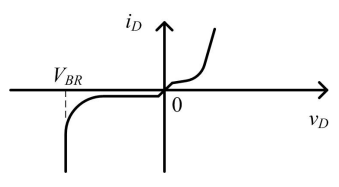
\includegraphics[width=0.9\linewidth]{Lab01/Lab1_diode_vi.png}
                        \caption{V-I Graph of Regular diodes}
                        \label{diode_vi}
                    \end{subfigure}
                    \hfill
                    \begin{subfigure}[h]{0.45\textwidth}
                        \centering
                        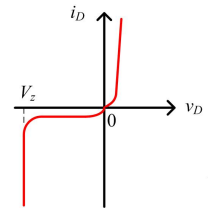
\includegraphics[width=0.6\linewidth]{Lab01/Lab1_zener_diode_vi.png}
                        \caption{V-I Graph of Zener diodes}
                        \label{z_diode_vi}
                    \end{subfigure}
                \end{figure}
                \FloatBarrier
                Diodes are widely used in electronic devices for tasks like rectification, circuit protection, and signal modulation.
                
            \item \textbf{Zener Diodes}\par
                Zener diode is the special type of diode, which is designed to allow current to flow in reverse direction when certain value of reverse voltage ($V_z$) is applied.
                
            \item \textbf{Schottky Diodes}\par
                Schottky diode is another specialized type of diode, it has a low forward voltage drop and a very fast switching action. Differ from diodes mentioned above, it is formed by the junction of a semiconductor with a metal.
        \end{itemize}
    \subsection{Specification}
        \begin{itemize}
            \item \hyperref[1N4148]{\textbf{Diode (1N4148)}}
            \item \hyperref[SR160]{\textbf{Schottky didode (SR160)}}
            \item \hyperref[1N4728A]{\textbf{Zener diode (1N4728A)}}
        \end{itemize}
    
\newpage
    \subsection{Circuit Diagram}
    \begin{figure}[h]

        \begin{subfigure}[h]{0.47\textwidth}
        \begin{center}
            \includesvg[width=1\linewidth]{Lab01/Lab1a.drawio.svg}
            \caption{}
            \label{Lab1a}
        \end{center} 
        \end{subfigure}
    \hfill
    \vspace{0.2 cm}
        \begin{subfigure}[h]{0.47\textwidth}
        \begin{center}
            \includesvg[width=1\linewidth]{Lab01/Lab1b.drawio.svg}
            \caption{}
            \label{Lab1b}
        \end{center}
        \end{subfigure}
    \vfill
    \vspace{0.2 cm}
        \begin{subfigure}[h]{0.47\textwidth}
        \begin{center}
            \includesvg[width=1\linewidth]{Lab01/Lab1c.drawio.svg} 
            \caption{}
            \label{Lab1c}
        \end{center}
        \end{subfigure}
    \hfill
        \begin{subfigure}[h]{0.47\textwidth}
        \begin{center}
            \includesvg[width=1\linewidth]{Lab01/Lab1d.drawio.svg}
            \caption{}
            \label{Lab1d}
        \end{center}
        \end{subfigure}
    \caption{Simlpe Diode Circuits}
    \label{SDC}

    \end{figure}
\FloatBarrier
The R shown in the circuits represents 1k$\Omega$. D is the unlabelled diode.


\section{Detailed Procedures}
    \subsection{Analyzation}
    First, we analyse the relationship between $V_s$ and $V_x$ and the theoretical value of each circuit.\par
    The relationship between $V_i$ and $V_o$ is:
    \begin{itemize}
        \item In figure. \ref{Lab1a}:
            \begin{itemize}
                \item When $V_s \ge V_\gamma$, D is on\par
                    $V_x = \frac{2}{3}V_s - V_\gamma$
                \item When $V_s \le V_\gamma$, D is off\par
                    $V_x = 0$
            \end{itemize}
        \item In figure. \ref{Lab1b}:
            \begin{itemize}
                \item 
            \end{itemize}
        \item In figure. \ref{Lab1c}:
            \begin{itemize}
                \item 
            \end{itemize}
        \item In figure. \ref{Lab1d}:
            \begin{itemize}
                \item 
            \end{itemize}
    \end{itemize}

    
    \subsection{Procedures}


\section{Discussion}


\section{Conclusion}

